
% VLDB template version of 2020-08-03 enhances the ACM template, version 1.7.0:
% https://www.acm.org/publications/proceedings-template
% The ACM Latex guide provides further information about the ACM template

\documentclass[sigconf, nonacm]{acmart}

%% The following content must be adapted for the final version
% paper-specific
\newcommand\vldbdoi{XX.XX/XXX.XX}
\newcommand\vldbpages{XXX-XXX}
% issue-specific
\newcommand\vldbvolume{14}
\newcommand\vldbissue{1}
\newcommand\vldbyear{2020}
% should be fine as it is
\newcommand\vldbauthors{\authors}
\newcommand\vldbtitle{\shorttitle} 
% leave empty if no availability url should be set
\newcommand\vldbavailabilityurl{URL_TO_YOUR_ARTIFACTS}
% whether page numbers should be shown or not, use 'plain' for review versions, 'empty' for camera ready
\newcommand\vldbpagestyle{plain} 
\usepackage{enumitem}
\usepackage{tabularx}
\usepackage{booktabs}
%\usepackage{algorithmic}
% Typography + line breaking
\usepackage{microtype}           % better kerning, fewer overfull boxes
\allowdisplaybreaks              % let AMS equations break across pages/columns
\clubpenalty=10000 \widowpenalty=10000 \displaywidowpenalty=10000

% Algorithms: modern and compact
\usepackage{algorithm}
\usepackage[noend]{algpseudocode}  % instead of 'algorithmic'
\algrenewcommand\algorithmicindent{0.8em}
\algrenewcommand{\algorithmicrequire}{\textbf{Input:}}
\algrenewcommand{\algorithmicensure}{\textbf{Output:}}

% Better control for wide floats in two columns (optional)
\usepackage{dblfloatfix}         % enables [b] for * floats under two-column
\usepackage{tikz}
\usetikzlibrary{arrows.meta,positioning}

\newtheorem{theorem}{Theorem}
\newtheorem{remark}{Remark}
\newtheorem{proposition}{Proposition}
\newtheorem{corollary}{Corollary}
\newtheorem{definition}{Definition}
\newtheorem{example}{Example}
\newtheorem{assumption}{Assumption}
\begin{document}
\title{From Local Summaries to Global Certificates: Predictive Memory Sizing for Distributed Heavy-Hitter Tracking}

%%
%% The "author" command and its associated commands are used to define the authors and their affiliations.
\author{Nikolaos Chalvantzis}
\affiliation{%
  \institution{National Technical University of Athens}
  \city{Athens}
  \country{Greece}
  }
\email{nchalv@cslab.ece.ntua.gr}

% \author{Lars Th{\o}rv{\"a}ld}
% \orcid{0000-0002-1825-0097}
% \affiliation{%
%   \institution{The Th{\o}rv{\"a}ld Group}
%   \streetaddress{1 Th{\o}rv{\"a}ld Circle}
%   \city{Hekla}
%   \country{Iceland}
% }
% \email{larst@affiliation.org}

% \author{Valerie B\'eranger}
% \orcid{0000-0001-5109-3700}
% \affiliation{%
%   \institution{Inria Paris-Rocquencourt}
%   \city{Rocquencourt}
%   \country{France}
% }
% \email{vb@rocquencourt.com}

% \author{J\"org von \"Arbach}
% \affiliation{%
%   \institution{University of T\"ubingen}
%   \city{T\"ubingen}
%   \country{Germany}
% }
% \email{jaerbach@uni-tuebingen.edu}
% \email{myprivate@email.com}
% \email{second@affiliation.mail}

% \author{Wang Xiu Ying}
% \author{Zhe Zuo}
% \affiliation{%
%   \institution{East China Normal University}
%   \city{Shanghai}
%   \country{China}
% }
% \email{firstname.lastname@ecnu.edu.cn}

% \author{Donald Fauntleroy Duck}
% \affiliation{%
%   \institution{Scientific Writing Academy}
%   \city{Duckburg}
%   \country{Calisota}
% }
% \affiliation{%
%   \institution{Donald's Second Affiliation}
%   \city{City}
%   \country{country}
% }
% \email{donald@swa.edu}

%%
%% The abstract is a short summary of the work to be presented in the
%% article.
% --- BEGIN inlined from sections_content/00_abstract.tex ---
\begin{abstract}
Modern distributed stream processing systems rely on partitioning to scale, but workload skew can severely degrade performance by overloading downstream workers. Identifying global heavy hitters is essential for mitigation, yet it remains a challenging coordinator-side inference problem when raw records cannot be centralized and local partition memory is strictly bounded. In this paper, we propose a unified framework for distributed heavy-hitter tracking that bridges deterministic inference and predictive memory provisioning. First, we introduce a routing-agnostic certification layer that converts bounded local Space-Saving telemetry into deterministic global frequency intervals. By explicitly decomposing coordinator error into reporter inflation and hidden non-reporter mass, we establish a strict discoverability floor that guarantees no global heavy hitter is missed. Second, we build a requirement-based predictive sizing controller on top of these certificates. Rather than forecasting abstract difficulty scores, our controller infers a retrospective required-capacity estimate expressed directly in units of memory. By modulating this requirement with the smoothed level and trend of heavy-hitter ambiguity, we generate a risk-adjusted effective signal that drives next-window provisioning. We also show how the same certification and planning logic extends to a hybrid exact-approximate regime that reserves exact state for stable dominant keys while tracking the residual tail approximately. Extensive evaluations demonstrate that our framework provides robust deterministic guarantees while optimizing the memory-quality tradeoff across highly volatile streams.
\end{abstract}
% --- END inlined from sections_content/00_abstract.tex ---

\maketitle

%%% do not modify the following VLDB block %%
%%% VLDB block start %%%
\pagestyle{\vldbpagestyle}
\begingroup\small\noindent\raggedright\textbf{PVLDB Reference Format:}\\
\vldbauthors. \vldbtitle. PVLDB, \vldbvolume(\vldbissue): \vldbpages, \vldbyear.\\
\href{https://doi.org/\vldbdoi}{doi:\vldbdoi}
\endgroup
\begingroup
\renewcommand\thefootnote{}\footnote{\noindent
This work is licensed under the Creative Commons BY-NC-ND 4.0 International License. Visit \url{https://creativecommons.org/licenses/by-nc-nd/4.0/} to view a copy of this license. For any use beyond those covered by this license, obtain permission by emailing \href{mailto:info@vldb.org}{info@vldb.org}. Copyright is held by the owner/author(s). Publication rights licensed to the VLDB Endowment. \\
\raggedright Proceedings of the VLDB Endowment, Vol. \vldbvolume, No. \vldbissue\ %
ISSN 2150-8097. \\
\href{https://doi.org/\vldbdoi}{doi:\vldbdoi} \\
}\addtocounter{footnote}{-1}\endgroup
%%% VLDB block end %%%

%%% do not modify the following VLDB block %%
%%% VLDB block start %%%
\ifdefempty{\vldbavailabilityurl}{}{
\vspace{.3cm}
\begingroup\small\noindent\raggedright\textbf{PVLDB Artifact Availability:}\\
The source code, data, and/or other artifacts have been made available at \url{\vldbavailabilityurl}.
\endgroup
}
%%% VLDB block end %%%
% --- BEGIN inlined from sections_content/01_introduction.tex ---
\section{Introduction}
\label{sec:introduction}

Modern distributed stream processing systems rely on input partitioning to scale keyed operators such as aggregations, joins, and stateful enrichments. This architecture is effective when the input is reasonably balanced, but it becomes fragile under skew, where a small number of keys accounts for a disproportionate share of the stream. Such keys can overload downstream workers, degrade latency, and undermine the effectiveness of otherwise well-provisioned execution pipelines. In many deployments, the ability to identify these dominant keys early is a prerequisite for mitigation mechanisms such as selective replication, routing overrides, or workload-aware state placement.

A natural object of interest is the set of \emph{global heavy hitters}: keys whose global relative frequency exceeds the balancing threshold induced by the number of downstream workers. Detecting such keys in a distributed stream, however, is fundamentally a coordinator-side inference problem. Each input partition observes only a fragment of the window, per-partition memory is bounded, and centralizing all raw records at the barrier is infeasible. A key that is globally important may appear only weakly, or not at all, in many local views. If it is omitted from all local summaries, it is unrecoverable. Thus, sketch sizing is not merely a question of compression efficiency; it is directly tied to discoverability and correctness.

This raises two closely related questions. First, given only compact local telemetry, what can a coordinator certify \emph{deterministically} about global heavy hitters in a realized window? Second, how should local sketch capacity be chosen for the \emph{next} window so that these guarantees remain useful under changing workloads? Existing sketching primitives provide local retention and frequency bounds, but the coordinator still needs a routing-agnostic way to turn those local guarantees into global certified conclusions. Likewise, adaptive provisioning should ideally be driven by a quantity that is directly meaningful for the actuator, rather than by an indirect notion of difficulty.

This paper addresses both questions through a unified framework built around local Space-Saving summaries. Our starting point is a deterministic coordinator-side certification layer: from local Space-Saving telemetry, the coordinator constructs a global candidate set, derives certified frequency intervals for reported keys, and partitions them into certified heavy hitters, certified non-heavy-hitters, and ambiguous keys. These guarantees are computed from the realized window only and require no stochastic routing assumptions. The key technical device is a signed decomposition of coordinator error into two components: \emph{reporter inflation}, caused by one-sided local overestimation, and \emph{hidden non-reporter mass}, caused by partitions that do not report a key. This decomposition yields explicit routing-agnostic envelopes and a simple discoverability floor under which no true heavy hitter can be missed at the candidate stage.

We then build the adaptive layer on top of these deterministic certificates. Rather than forecasting an abstract difficulty statistic and then inverting that forecast into a sketch size, we introduce a \emph{requirement-based} view of provisioning. For a realized window, we ask a direct question: under the deterministic envelope model, what sketch capacity does the model prescribe for satisfying a target margin? This yields a window-level \emph{required capacity} signal, expressed in the same units as the memory actuator itself. The signal is a conservative retrospective estimate, not an exact counterfactual minimum, but it avoids forecasting an abstract surrogate that must later be mapped into memory through a separate response model. This viewpoint produces a cleaner planning layer, a more interpretable controller, and a sharper separation between deterministic within-window inference and probabilistic cross-window adaptation.

The result is a two-layer architecture. The first layer provides deterministic coordinator-side guarantees for a realized window. The second uses the output of the first to plan memory for the next window. This separation is important both conceptually and operationally. It ensures that correctness claims about the realized window do not depend on the success of forecasting, while still allowing the system to adapt its memory footprint over time. Ambiguity near the heavy-hitter boundary can be incorporated as a secondary guardrail, but it does not replace required capacity as the main planning variable.

Our contributions are as follows:
\begin{itemize}[leftmargin=*]
    \item We develop a deterministic coordinator-side certification framework that converts local Space-Saving telemetry into routing-agnostic global frequency intervals, together with certified heavy hitters, certified non-heavy-hitters, and ambiguous keys.
    \item We establish a simple discoverability guarantee: above a natural per-partition size floor, every global heavy hitter is guaranteed to appear in the coordinator's candidate set, eliminating false negatives at the discovery stage.
    \item We introduce a requirement-based formulation of adaptive sizing. From the deterministic margins observed in a realized window, we infer a conservative memory-valued estimate of the sketch capacity needed to satisfy a prescribed service target under the certification model.
    \item We build a predictive next-window sizing policy on top of this required-capacity signal, and show how ambiguity-aware control and hybrid exact-approximate tracking fit naturally within the same architecture.
\end{itemize}

The rest of the paper is organized as follows. Section~\ref{sec:problem} formalizes the system model and coordinator interface. Section~\ref{sec:ss-prelim} presents the local Space-Saving primitive and the telemetry contract. Section~\ref{sec:deterministic} develops deterministic coordinator-side certification for global heavy hitters. Section~\ref{sec:requirement} introduces the requirement-based view of memory sizing. Section~\ref{sec:predictive} presents the predictive next-window controller. Section~\ref{sec:extensions} extends the framework to hybrid exact-approximate tracking, and Section~\ref{sec:experiments} outlines the experimental evaluation.

\section{System Model and Coordinator Interface}
\label{sec:problem}
\begin{figure*}[t]
\centering
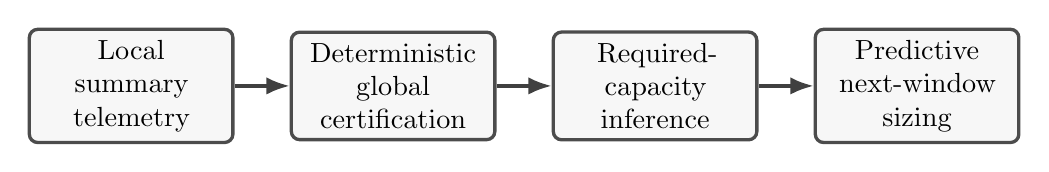
\begin{tikzpicture}[
    node distance=0.7cm,
    >=Latex,
    every node/.style={align=center},
    box/.style={
        draw=black!70,
        rounded corners=3pt,
        very thick,
        minimum height=1.1cm,
        text width=0.19\textwidth,
        inner sep=4pt,
        fill=black!3
    },
    flow/.style={
        ->,
        very thick,
        draw=black!75
    },
    group/.style={
        draw=black!35,
        rounded corners=4pt,
        fill=black!1,
        inner sep=8pt
    },
    grouplabel/.style={
        font=\small\bfseries,
        text=black!75
    }
]

\node[box] (telemetry) {Local summary\\telemetry};
\node[box, right=of telemetry] (certs) {Deterministic\\global certification};
\node[box, right=of certs] (req) {Required-capacity\\inference};
\node[box, right=of req] (predictive) {Predictive\\next-window sizing};

\draw[flow] (telemetry) -- (certs);
\draw[flow] (certs) -- (req);
\draw[flow] (req) -- (predictive);
\end{tikzpicture}
\caption{Conceptual pipeline of the proposed framework. The coordinator converts bounded local summary telemetry into deterministic global certificates for the realized window, then inverts those certificates into a required-capacity signal that drives predictive sizing for the next window.}
\Description{A four-stage left-to-right pipeline: local summary telemetry, deterministic global certification, required-capacity inference, and predictive next-window sizing.}
\label{fig:pipeline}
\end{figure*}

We consider a windowed distributed stream processing system that ingests a high-rate key--value stream and executes keyed operators over \(n\) parallel downstream workers. Input arrives through \(m\) disjoint input partitions. These two roles are deliberately separated. Input partitions observe local fragments of the stream and emit compact telemetry at window boundaries, while downstream workers are the entities whose load balance motivates the heavy-hitter threshold. The setting is representative of modern streaming deployments in which raw records cannot be centralized continuously, yet coordinator-side decisions must still be made from bounded summary state.

Processing proceeds in fixed, non-overlapping windows indexed by \(t \in \mathbb{N}\). Let \(\mathcal W^t\) denote the multiset of all records arriving in window \(t\), and let \(N^t = |\mathcal W^t|\) be its total mass. Partition \(i \in [m]\) observes a local substream \(\mathcal W_i^t\) with mass \(N_i^t = |\mathcal W_i^t|\), where \(\sum_{i=1}^m N_i^t = N^t\). We make no assumptions about how the stream is split across partitions: the system may experience arbitrary imbalance both across partitions and across windows. Each record carries a key \(k \in \mathcal{K}\), where \(\mathcal{K}\) is the key universe. We analyze nonempty windows \(N^t>0\); an empty global window contains no heavy hitters and all certification statements are vacuous. Let
\[
\mathcal A^t := \{\, i \in [m] : N_i^t>0 \,\}
\]
denote the set of active partitions in window \(t\). We write \(f^t(k)\) and \(f_i^t(k)\) for the global and local counts of key \(k\), and we write
\[
p^t(k) := \frac{f^t(k)}{N^t},
\qquad
p_i^t(k) := \frac{f_i^t(k)}{N_i^t}
\]
for the corresponding global relative frequency and, when \(i\in\mathcal A^t\), local relative frequency. For inactive partitions \(i\notin\mathcal A^t\), all local counts are zero and \(p_i^t(k)\) is not used; their summaries contribute only zero mass and zero minimum-counter terms under the conventions below. Unless ambiguity would arise, we suppress the superscript \(t\) when the reference window is clear.

The paper is concerned with \emph{global heavy hitters}, that is, keys whose global frequency exceeds the natural balancing threshold induced by the number of downstream workers.

\begin{definition}[Global heavy hitter]
\label{def:hh}
A key \(k \in \mathcal{K}\) is a global heavy hitter in window \(t\) if
\[
p^t(k) > \frac{1}{n}.
\]
We denote the set of global heavy hitters by
\[
\mathcal{H}_n^t := \left\{ k \in \mathcal{K} : p^t(k) > \frac{1}{n} \right\}.
\]
\end{definition}

This threshold is operationally meaningful: a key whose mass exceeds \(1/n\) cannot be evenly absorbed by \(n\) downstream workers without some form of special treatment. This is the canonical balancing threshold for keyed downstream execution over \(n\) workers. More complex downstream operators may induce different operational thresholds, but such cases are outside the scope of the present paper. The heavy-hitter set is also small in a worst-case sense.

\begin{proposition}[Cardinality bound]
\label{prop:hh-count}
For every window \(t\),
\[
|\mathcal{H}_n^t| < n.
\]
\end{proposition}

\begin{proof}
If \(\{k_1,\dots,k_r\} \subseteq \mathcal{K}\) and \(p^t(k_j) > 1/n\) for all \(j\), then
\[
1
=
\sum_{k \in \mathcal{K}} p^t(k)
\ge
\sum_{j=1}^r p^t(k_j)
>
\frac{r}{n},
\]
hence \(r < n\).
\end{proof}

This bound is purely combinatorial and holds regardless of skew or partitioning. In realistic workloads, the number of global heavy hitters is often much smaller than \(n\), but the worst-case bound provides a useful scale for certification and provisioning.

The coordinator's per-window task has two parts. First, it must ensure \emph{discoverability}: every global heavy hitter should appear in at least one local report, so that it is not lost before global inference even begins. Second, for every reported key, it should derive deterministic frequency bounds strong enough to support certified heavy-hitter decisions.

To support this inference task, each input partition maintains a bounded local summary over its local window and emits only compact telemetry at the barrier. The main regime studied in the paper uses a single fixed-size summary per partition; the specific summary primitive is introduced in Section~\ref{sec:ss-prelim}. At this level of abstraction, what matters is that partition \(i\) exports its local window mass \(N_i^t\), a bounded dictionary of retained keys with summary-specific metadata, and a small amount of scalar telemetry that allows the coordinator to reason about keys that were \emph{not} retained locally. The coordinator never sees raw records. Its view of the window is entirely mediated by this telemetry contract.

From the summaries received at the barrier, the coordinator forms a global candidate set \(\mathcal{U}^t\), consisting of all keys reported by at least one partition. It then computes, for each \(k \in \mathcal{U}^t\), a deterministic interval
\[
[\underline p^t(k), \overline p^t(k)]
\]
that encloses the true global frequency \(p^t(k)\). These intervals support a three-way partition of the candidate set into certified heavy hitters, certified non-heavy-hitters, and ambiguous keys. The concrete construction of \(\mathcal{U}^t\) and of these deterministic envelopes depends on the local summary primitive and is developed later; for now, the important point is that coordinator-side inference is driven entirely by bounded telemetry emitted at the barrier.

A central organizational principle of the paper is the separation between \emph{realized-window certification} and \emph{next-window planning}. Once a window has completed and all local telemetry has been received, the coordinator-side guarantees derived in this paper are deterministic. They do not rely on routing randomness, temporal smoothness, or workload stationarity. By contrast, choosing memory for the next window is inherently predictive: it requires extrapolating from what was observed in window \(t\) to what may happen in window \(t+1\). This distinction is not merely expository. It is what allows the paper to make strong correctness claims about the realized window while treating adaptation as a separate, explicitly predictive layer. If the system mis-sizes a future window, the realized-window certificates remain valid; only the sharpness of the next round of inference is affected.

The output of the realized-window layer is therefore concrete and finite. For each window \(t\), the coordinator returns the candidate set \(\mathcal{U}^t\), deterministic frequency intervals for all candidates, and a partition of candidates into certified positives, certified negatives, and ambiguous keys. Together, these objects form the coordinator-side certificate for the realized window. The planning layer then uses those same certificates to infer a memory-valued requirement estimate for the realized window, and to convert that estimate into a sizing decision for the next window. Figure~\ref{fig:pipeline} summarizes this architecture.

Table~\ref{tab:notation} summarizes the main notation used throughout the paper.

\begin{table}[t]
\centering
\caption{Main notation. Time superscripts are omitted when the reference window is clear from context.}
\label{tab:notation}
\scriptsize
\setlength{\tabcolsep}{3pt}
\renewcommand{\arraystretch}{0.96}
\begin{tabularx}{\columnwidth}{@{}lX@{}}
\toprule
\textbf{Symbol} & \textbf{Meaning} \\
\midrule
\multicolumn{2}{@{}l}{\textit{System and stream model}} \\
\midrule
\(n,m\) & Number of downstream workers (\(n\)) and input partitions (\(m\)) \\
\(\mathcal K\) & Universe of possible keys \\
\(\mathcal W,\mathcal W_i\) & Global window multiset and partition-\(i\) local substream \\
\(N,N_i,\mathcal A\) & Global window mass, partition-local mass, and active partitions \(\{i:N_i>0\}\) \\
\(f(k),f_i(k)\) & Global and local counts of key \(k\) \\
\(p(k),p_i(k)\) & Global and local relative frequencies of key \(k\) \\
\(\mathcal H_n\) & Global heavy-hitter set \(\{k:p(k)>1/n\}\) \\
\midrule
\multicolumn{2}{@{}l}{\textit{Local summaries and coordinator observables}} \\
\midrule
\(\mathcal S_i,q\) & Partition-\(i\) Space-Saving summary and its common local capacity \\
\(\hat f_i(k),\varepsilon_i(k)\) & Local estimate of key \(k\) and its one-sided overestimation certificate \\
\(c_i\) & Final minimum-counter bound of partition \(i\); also the bound used for hidden non-reporter mass \\
\(\mathcal U\) & Union of keys reported by at least one partition in the realized window \\
\(R(k)\) & Set of partitions whose local summaries report key \(k\) \\
\(\hat f(k),\hat p(k)\) & Coordinator aggregate count estimate and corresponding relative-frequency estimate \\
\midrule
\multicolumn{2}{@{}l}{\textit{Deterministic certification}} \\
\midrule
\(\underline p(k),\overline p(k)\) & Deterministic lower and upper bounds on the true global relative frequency \(p(k)\) \\
\(K_+,K_-,K_?\) & Certified heavy hitters, certified non-heavy-hitters, and ambiguous candidates \\
\(T\) & HH-relevant target set \(K_+ \cup K_?\) used by the planning layer \\
\(I(k),H(k),M(k)\) & Reporter-inflation term, hidden-mass term, and composite deterministic margin \\
\midrule
\multicolumn{2}{@{}l}{\textit{Planning and predictive control}} \\
\midrule
\(r_M\) & Target deterministic margin budget for HH-relevant keys \\
\(q_{\mathrm{req}}(k),q_{\mathrm{Req}}\) & Per-key required capacity and window-level required-capacity signal \\
\(D_A,\bar D_A,G_A\) & Ambiguity ratio, smoothed ambiguity level, and signed ambiguity trend \\
\(\lambda_A,\lambda_G\) & Controller gains for ambiguity level and ambiguity trend \\
\(z_{\mathrm{eff}},q_{\mathrm{eff}}\) & Log effective signal and ambiguity-adjusted effective memory signal \\
\(\hat z_{\mathrm{eff}},R_{\mathrm{eff}},b_{\mathrm{eff}}\) & One-step log forecast, forecast residual, and one-sided calibration bias \\
\(\tilde z_{\mathrm{eff}},\tilde q_{\mathrm{eff}}\) & Calibrated log forecast and calibrated next-window effective signal \\
\(q_{\mathrm{react,Req}},q_{\mathrm{react,eff}}\) & Reactive requirement-replay and effective-signal-replay baselines \\
\(q\) & Deployed common local summary size in the core regime \\
\midrule
\multicolumn{2}{@{}l}{\textit{Hybrid exact--approximate tracking}} \\
\midrule
\(E,q_e,q_a,q_{\mathrm{hyb}}\) & Promoted exact head, exact-head size, residual approximate-summary size, and total hybrid local memory \\
\(\mathcal W_{i,\mathrm{res}},\mathcal S_{i,\mathrm{res}}\) & Residual substream and residual Space-Saving summary at partition \(i\) \\
\(N_{\mathrm{res}},N_{i,\mathrm{res}},\mathcal A_{\mathrm{res}}\) & Global residual mass, partition-local residual mass, and residual-active partitions \\
\(P_E\) & Fraction of global mass captured exactly by the promoted head \(E\) \\
\(R_{\mathrm{res}}(k),c_{i,\mathrm{res}}\) & Residual reporting set of key \(k\) and residual minimum-counter bound at partition \(i\) \\
\(\underline p_{\mathrm{res}}(k),\overline p_{\mathrm{res}}(k)\) & Deterministic residual frequency bounds for keys outside the exact head \\
\(q_{\mathrm{res},\min}\) & Residual discoverability floor in the hybrid regime \\
\bottomrule
\end{tabularx}
\end{table}



The remainder of the paper develops this pipeline in stages. Section~\ref{sec:ss-prelim} introduces the local summary primitive and the telemetry it exposes. Section~\ref{sec:deterministic} shows how the coordinator converts that telemetry into deterministic global certificates. Section~\ref{sec:requirement} then turns those certificates into a window-level required-capacity signal, and Section~\ref{sec:predictive} uses that signal for predictive memory sizing. A hybrid exact--approximate regime is treated as an extension rather than as part of the core theorem path.

\section{Local Space-Saving Summaries and Telemetry}
\label{sec:ss-prelim}

This section introduces the local summary primitive used throughout the paper and isolates the properties that will later support coordinator-side certification. Our main regime assigns one bounded summary to each input partition in each window. The purpose of the summary is not merely to compress local frequency information, but to expose enough structure at the barrier for a coordinator to reason deterministically about the global stream.


We use \emph{Space-Saving} (SS) as the local primitive, implemented faithfully via the original \emph{Stream-Summary} data structure of Metwally et al.~\cite{metwally2005efficient}. In our setting, each partition maintains one such summary per window and exports its end-of-window telemetry at the barrier. Space-Saving is well suited to this role for three reasons. First, it retains explicitly named keys rather than only hashed counters, which makes coordinator-side aggregation and certification possible without an additional key-recovery mechanism. Second, it provides a deterministic local retention threshold: any key whose local relative frequency exceeds \(1/q\) must appear in a summary of size \(q\). Third, every retained key is accompanied by a one-sided frequency certificate, while the minimum counter in the final summary gives a direct bound on the mass of any key that was not retained locally. These are precisely the ingredients needed in the next section to separate coordinator error into inflation from reporting partitions and hidden mass from non-reporting ones.

\subsection{Partition-Local Summary Primitive}
\label{subsec:ss-algorithm}

Fix a window \(t\) and a partition \(i\). The partition processes its local substream \(\mathcal W_i^t\) using a Space-Saving summary \(\mathcal{S}_i^t\) of capacity \(q^t\). The summary stores at most \(q^t\) keys. For each retained key \(k\), it maintains an estimated local count \(\hat f_i^t(k)\) together with a nonnegative overestimation certificate \(\varepsilon_i^t(k)\).

The update rule is standard. When an item with key \(k\) arrives, the summary increments the existing counter if \(k\) is already present. If \(k\) is absent and free capacity remains, the summary inserts \(k\) with unit count and zero error. Otherwise, the summary replaces the currently minimum counter entry: the evicted key is discarded, the incoming key takes its place, its new counter is set to one plus the minimum counter that was evicted, and that minimum counter is recorded as the new key's error certificate.

\begin{algorithm}[t]
\caption{Space-Saving update at partition \(i\)}
\label{alg:ss-update}
\small
\begin{algorithmic}[1]
\Require Summary \(\mathcal{S}\) with capacity \(q\), incoming key \(k\)
\If{\(k \in \mathcal{S}\)}
    \State \(\hat f(k) \gets \hat f(k)+1\)
\ElsIf{\(|\mathcal{S}|<q\)}
    \State insert \(k\) with \(\hat f(k)\gets 1\) and \(\varepsilon(k)\gets 0\)
\Else
    \State \(x \gets \arg\min_{u \in \mathcal{S}} \hat f(u)\)
    \State replace \(x\) by \(k\)
    \State \(\hat f(k)\gets \hat f(x)+1\)
    \State \(\varepsilon(k)\gets \hat f(x)\)
\EndIf
\end{algorithmic}
\end{algorithm}

The implementation used in this paper is faithful to the original Space-Saving design of Metwally et al. Specifically, each local summary is realized as a \emph{Stream-Summary}, which groups items of equal estimated count into buckets maintained in sorted order. Monitored items are accessed directly through a hash table (or equivalent associative structure), while counter increments are handled by moving items between adjacent buckets as their estimated counts change. This representation supports constant-time lookup of monitored items together with lightweight local updates.

While the coordinator-side analysis depends only on the end-of-window invariants exposed by Stream-Summary, our local implementation remains faithful to the original Space-Saving design.

\subsection{Summary Invariants}
\label{subsec:ss-invariants}

We now record the properties of Space-Saving that the coordinator will later use. For readability, we suppress the window superscript \(t\) in this subsection.

The first property is the familiar one-sided certificate for retained keys.

\begin{lemma}[One-sided local certificate]
\label{lem:ss-certificate}
For any partition \(i\) and any key \(k \in \mathrm{keys}(\mathcal{S}_i)\),
\[
f_i(k) \le \hat f_i(k) \le f_i(k)+\varepsilon_i(k),
\qquad
0 \le \varepsilon_i(k) \le c_i \le \frac{N_i}{q},
\]
where
\[
c_i :=
\begin{cases}
0, & |\mathrm{keys}(\mathcal S_i)| < q,\\[0.75ex]
\min_{x \in \mathrm{keys}(\mathcal{S}_i)} \hat f_i(x), & |\mathrm{keys}(\mathcal S_i)| = q.
\end{cases}
\]
Equivalently, \(c_i\) is the minimum over the \(q\) logical counters of the summary, treating unused counters as zero.
\end{lemma}

Thus the local estimate of a retained key never underestimates its true local count, and any overestimation is explicitly bounded. This one-sidedness is essential later: it ensures that partitions reporting a key can only contribute upward error to the coordinator.

The second property is the deterministic retention threshold.

\begin{lemma}[Deterministic local retention]
\label{lem:ss-retention}
For a partition \(i\) with \(N_i>0\), let \(\tau = 1/q\). If a key \(k\) satisfies
\[
p_i(k)=\frac{f_i(k)}{N_i}>\tau,
\]
then \(k\) must belong to the retained key set \(\mathrm{keys}(\mathcal{S}_i)\).
\end{lemma}

This lemma is the basis of the discoverability result in Section~\ref{sec:deterministic}. It converts a local support condition into a deterministic statement about visibility at the coordinator.

The third property concerns keys that are \emph{not} present in the final local summary.

\begin{lemma}[Absence bound via the minimum counter]
\label{lem:ss-mincounter}
For any partition \(i\) and any key \(k \notin \mathrm{keys}(\mathcal{S}_i)\),
\[
f_i(k) \le c_i.
\]
In particular,
\[
c_i \le \frac{N_i}{q}.
\]
\end{lemma}

\begin{proof}
If the summary is not full at the end of the window, no eviction has occurred, every key with positive local count is retained, and \(c_i=0\). Hence any absent key has \(f_i(k)=0\). If the summary is full, the first inequality is the standard Space-Saving absence invariant: any key that is not retained at the end can have accumulated no more mass than the final minimum counter. Otherwise, its local frequency would have forced it to displace some retained key. The second inequality follows because, in the full case, the \(q\) retained counters sum to \(N_i\), so their minimum cannot exceed their average \(N_i/q\).
\end{proof}

This minimum counter plays a central role in the coordinator analysis. It does more than certify which keys were retained; it also gives the coordinator a uniform worst-case bound on the local mass of every key that was \emph{not} retained. Thus \(c_i\) is precisely the scalar that later bounds the hidden non-reporter mass: if partition \(i\) does not report key \(k\), then the coordinator may still charge up to \(c_i\) units of unseen local mass to \(k\), but no more. As a result, non-reporting partitions remain visible to the coordinator through a scalar quantity, even when they do not explicitly mention a given key.

Finally, the update rule preserves an exact accounting identity that is useful for implementation sanity checks and for interpreting the summary as a partition-local compression of the full window.

\begin{lemma}[Counter-sum identity]
\label{lem:ss-sum}
At the end of the window,
\[
\sum_{x \in \mathrm{keys}(\mathcal{S}_i)} \hat f_i(x) = N_i.
\]
\end{lemma}

Every arriving item increments exactly one counter, so the sum of the retained counters equals the total local mass processed by the summary.

Taken together, Lemmas~\ref{lem:ss-certificate}--\ref{lem:ss-mincounter} provide the exact interface needed by the coordinator. Reporting partitions contribute explicit one-sided overestimation bounds, while non-reporting partitions contribute only bounded hidden mass through their minimum counters.

\subsection{Barrier Telemetry}
\label{subsec:ss-telemetry}

We treat end-of-window communication as an explicit telemetry contract between each input partition and the coordinator. The contract is window-local: partitions export only compact information derived from the realized window, and no temporal state is required for the deterministic certification layer.

At the end of window \(t\), partition \(i\) transmits its local window mass \(N_i^t\) together with the contents of its Space-Saving summary,
\[
\mathcal{S}_i^t
=
\left\{
\bigl(k,\hat f_i^t(k),\varepsilon_i^t(k)\bigr)
:\;
k \text{ retained locally}
\right\},
\qquad
|\mathcal{S}_i^t| \le q^t.
\]
The partition may also transmit the minimum counter
\[
c_i^t :=
\begin{cases}
0, & |\mathcal S_i^t| < q^t,\\[0.75ex]
\min_{x \in \mathrm{keys}(\mathcal{S}_i^t)} \hat f_i^t(x), & |\mathcal S_i^t| = q^t,
\end{cases}
\]
which is the final minimum over the \(q^t\) logical counters, treating unused counters as zero. In practice, this value is derivable from the transmitted dictionary itself with a single \(O(q^t)\) scan per partition at the barrier. Once computed, it is reused in all coordinator-side envelope calculations for that window. No raw local records are exported.

This telemetry is sufficient for all coordinator-side tasks in the core framework. From the union of locally retained keys, the coordinator forms a candidate set for the realized window. From the reported estimates and certificates, it computes deterministic lower and upper bounds for each candidate's global frequency. From the per-partition minimum counters, it bounds the hidden mass contributed by partitions that do not report a candidate. The same telemetry therefore supports both discoverability arguments and quantitative frequency envelopes.

It is important to emphasize what the coordinator is \emph{not} assumed to do. The coordinator is not required to merge local Space-Saving summaries into a new valid Space-Saving instance for continued streaming use. In the present paper it acts as a terminal sink for window-level inference: it consumes local telemetry, produces deterministic certificates for the realized window, and emits planning signals for the next one. This choice keeps the reasoning faithful to the barriered streaming setting and avoids introducing an unnecessary mergeability requirement into the theorem path.

Section~\ref{sec:problem} defined the system model and the coordinator interface at a high level. The present section makes that interface concrete by identifying the local primitive and the invariants it exposes. The next section uses these invariants to derive the main deterministic results of the paper: a discoverability floor for global heavy hitters, a signed decomposition of coordinator-side error, and explicit routing-agnostic frequency intervals for all reported candidates.

\section{Deterministic Global Heavy-Hitter Certification}
\label{sec:deterministic}

We now turn to the main inference problem of the paper. At the end of a realized window, the coordinator receives bounded telemetry from all partitions and must reason about global heavy hitters without access to raw records. The goal of this section is to show that the local invariants of Section~\ref{sec:ss-prelim} are already strong enough to support routing-agnostic global certification. Specifically, we establish three results. First, above a simple size floor, every global heavy hitter is guaranteed to appear in the coordinator's candidate set. Second, for every reported candidate, the coordinator can derive an explicit deterministic interval for its true global relative frequency. Third, these intervals induce a sound partition of candidates into certified heavy hitters, certified non-heavy-hitters, and ambiguous keys.

\subsection{Coordinator Aggregation}
\label{subsec:coord-aggregation}

Fix a realized window \(t\). Each partition \(i \in [m]\) exports its local mass \(N_i^t\), its Space-Saving summary \(\mathcal S_i^t\), and the associated end-of-window certificates described in Section~\ref{sec:ss-prelim}. The coordinator begins by forming the union of all locally reported keys:
\[
\mathcal U^t
:=
\bigcup_{i=1}^m \mathrm{keys}(\mathcal S_i^t).
\]
This is the candidate set for the realized window. Every key outside \(\mathcal U^t\) is absent from every local summary and must therefore be handled only indirectly through the minimum-counter bounds of non-reporting partitions.

For any candidate \(k \in \mathcal U^t\), define its reporting set by
\[
R^t(k)
:=
\{\, i \in [m] : k \in \mathrm{keys}(\mathcal S_i^t) \,\}.
\]
The coordinator's natural aggregate estimate of the global count of \(k\) is then
\[
\hat f^t(k)
:=
\sum_{i \in R^t(k)} \hat f_i^t(k),
\qquad
\hat p^t(k)
:=
\frac{\hat f^t(k)}{N^t},
\qquad
N^t := \sum_{i=1}^m N_i^t.
\]
This aggregate uses only the partitions that explicitly report \(k\). The key question is therefore how to account for the partitions in \([m]\setminus R^t(k)\), which do not report \(k\) but may still contain some of its mass.

\subsection{Discoverability Guarantee}
\label{subsec:discoverability}

We first establish the candidate-discovery guarantee. The coordinator can only certify a heavy hitter once that key appears in \(\mathcal U^t\), so the first concern is whether a true heavy hitter can be absent from every local summary.

\begin{proposition}[Discoverability floor]
\label{prop:discoverability}
If the common local summary size in window \(t\) satisfies
\[
q^t \ge n,
\]
then every global heavy hitter \(k \in \mathcal H_n^t\) appears in the candidate set \(\mathcal U^t\).
\end{proposition}

\begin{proof}
Let \(k\) be a global heavy hitter, so that \(p^t(k) > 1/n\). Suppose, for contradiction, that
\[
p_i^t(k) \le \frac{1}{n}
\qquad
\text{for all } i \in \mathcal A^t.
\]
Inactive partitions have \(f_i^t(k)=0\), so
\[
f^t(k)
=
\sum_{i=1}^m f_i^t(k)
\le
\sum_{i=1}^m \frac{N_i^t}{n}
=
\frac{N^t}{n},
\]
which implies \(p^t(k) \le 1/n\), a contradiction. Hence there exists some active partition \(i\in\mathcal A^t\) such that
\[
p_i^t(k) > \frac{1}{n}.
\]
If \(q^t \ge n\), then \(1/q^t \le 1/n\), and therefore
\[
p_i^t(k) > \frac{1}{q^t}.
\]
By Lemma~\ref{lem:ss-retention}, \(k\) must belong to \(\mathrm{keys}(\mathcal S_i^t)\), and thus \(k \in \mathcal U^t\).
\end{proof}

This proposition is the coordinator-side analogue of the local retention threshold. It says that once the local summary size reaches the balancing threshold \(n\), the discovery stage itself introduces no false negatives for global heavy hitters. This floor is tight for the worst-case visibility pattern: if a global heavy hitter distributes its mass as evenly as possible across partitions, then the most informative partition may see it at local relative frequency only slightly above \(1/n\), so the local retention threshold \(1/q^t\) must not exceed \(1/n\), which is exactly the condition \(q^t \ge n\). The condition is therefore sufficient, not necessary, for discoverability; in many realized windows, a global heavy hitter is much more concentrated than this worst case and remains discoverable even under smaller local summaries.

\subsection{Deterministic Frequency Envelopes}
\label{subsec:freq-envelopes}

We now derive deterministic frequency intervals for the candidates in \(\mathcal U^t\). The central observation is that coordinator-side error has a natural signed decomposition. For a candidate \(k \in \mathcal U^t\),
\[
\hat f^t(k) - f^t(k)
=
\sum_{i \in R^t(k)} \bigl(\hat f_i^t(k) - f_i^t(k)\bigr)
-
\sum_{j \notin R^t(k)} f_j^t(k).
\]
The first term is the upward error contributed by reporting partitions. The second term is the hidden mass contributed by non-reporting partitions. These two terms are controlled by different summary invariants.

For reporting partitions, Lemma~\ref{lem:ss-certificate} gives
\[
0
\le
\hat f_i^t(k) - f_i^t(k)
\le
\varepsilon_i^t(k).
\]
For non-reporting partitions, Lemma~\ref{lem:ss-mincounter} gives
\[
f_j^t(k)
\le
c_j^t,
\]
where \(c_j^t\) is the transmitted minimum-counter bound defined in Section~\ref{subsec:ss-telemetry}.
Combining these bounds yields the following deterministic envelope.

\begin{proposition}[Deterministic global envelope]
\label{prop:global-envelope}
For every candidate \(k \in \mathcal U^t\),
\[
-\sum_{j \notin R^t(k)} c_j^t
\;\le\;
\hat f^t(k) - f^t(k)
\;\le\;
\sum_{i \in R^t(k)} \varepsilon_i^t(k).
\]
Equivalently,
\[
\hat f^t(k) - \sum_{i \in R^t(k)} \varepsilon_i^t(k)
\;\le\;
f^t(k)
\;\le\;
\hat f^t(k) + \sum_{j \notin R^t(k)} c_j^t.
\]
\end{proposition}

\begin{proof}
The result follows directly from the signed decomposition above together with the one-sided local certificates for \(i \in R^t(k)\) and the minimum-counter absence bounds for \(j \notin R^t(k)\).
\end{proof}

The upper bound intentionally contains no subtraction for reporting partitions. For a reporting partition \(i\in R^t(k)\), the true local count \(f_i^t(k)\) may be anywhere between \(\hat f_i^t(k)-\varepsilon_i^t(k)\) and \(\hat f_i^t(k)\); when maximizing the global frequency, the worst case is zero reporter-side overcount, so the contribution is simply \(\hat f_i^t(k)\). The only additional mass that can raise the global count beyond the aggregate reported estimate comes from partitions that did not report \(k\), and Lemma~\ref{lem:ss-mincounter} bounds each such hidden contribution by \(c_j^t\).

After normalization by \(N^t\), Proposition~\ref{prop:global-envelope} yields an explicit deterministic interval for the global relative frequency of every candidate:
\begin{align}
\underline p^t(k)
&:=
\max\!\left\{
0,\;
\hat p^t(k)
-
\frac{1}{N^t}
\sum_{i \in R^t(k)} \varepsilon_i^t(k)
\right\},
\label{eq:lower-envelope}
\\[0.75ex]
\overline p^t(k)
&:=
\min\!\left\{
1,\;
\hat p^t(k)
+
\frac{1}{N^t}
\sum_{j \notin R^t(k)} c_j^t
\right\}.
\label{eq:upper-envelope}
\end{align}

\begin{corollary}[Deterministic frequency interval]
\label{cor:freq-interval}
For every candidate \(k \in \mathcal U^t\),
\[
p^t(k) \in [\underline p^t(k), \overline p^t(k)].
\]
\end{corollary}

The interval remains valid even when some partitions are empty or very small. Empty partitions have zero local mass and, by convention, zero minimum counter; small partitions contribute only their realized minimum-counter terms. The resulting bound may be loose, but it remains sound.

These intervals are the main quantitative output of the realized-window certification layer. They are routing-agnostic, depend only on the observed telemetry, and remain valid regardless of whether the next window is ultimately provisioned correctly or not.

\subsection{Certification Partition}
\label{subsec:cert-partition}

The intervals derived above support a three-way partition of the candidate set. Define
\begin{align}
K_+^t
&:=
\{\, k \in \mathcal U^t : \underline p^t(k) > 1/n \,\},
\label{eq:kplus}
\\[0.75ex]
K_-^t
&:=
\{\, k \in \mathcal U^t : \overline p^t(k) \le 1/n \,\},
\label{eq:kminus}
\\[0.75ex]
K_?^t
&:=
\mathcal U^t \setminus (K_+^t \cup K_-^t).
\label{eq:kamb}
\end{align}
Thus \(K_+^t\) contains candidates that are certifiably heavy, \(K_-^t\) contains candidates that are certifiably non-heavy, and \(K_?^t\) contains those whose true status remains unresolved by the available telemetry.

\begin{proposition}[Soundness of the certification partition]
\label{prop:partition-sound}
For every realized window \(t\):
\begin{enumerate}[leftmargin=*]
    \item if \(k \in K_+^t\), then \(p^t(k) > 1/n\);
    \item if \(k \in K_-^t\), then \(p^t(k) \le 1/n\).
\end{enumerate}
\end{proposition}

\begin{proof}
If \(k \in K_+^t\), then \(\underline p^t(k) > 1/n\). Since \(p^t(k) \ge \underline p^t(k)\) by Corollary~\ref{cor:freq-interval}, it follows that \(p^t(k) > 1/n\). Similarly, if \(k \in K_-^t\), then \(\overline p^t(k) \le 1/n\), and since \(p^t(k) \le \overline p^t(k)\), we obtain \(p^t(k) \le 1/n\).
\end{proof}

The partition is therefore sound on both sides: certified positives are true heavy hitters, and certified negatives are true non-heavy-hitters. Ambiguity is the only place where the telemetry leaves room for uncertainty.

When the discoverability floor of Proposition~\ref{prop:discoverability} is enforced, this candidate-side partition lifts to a statement about the full heavy-hitter set.

\begin{corollary}[No false negatives under the discoverability floor]
\label{cor:no-false-negatives}
If \(q^t \ge n\), then every global heavy hitter belongs to \(K_+^t \cup K_?^t\).
\end{corollary}

\begin{proof}
By Proposition~\ref{prop:discoverability}, every global heavy hitter belongs to \(\mathcal U^t\). By Proposition~\ref{prop:partition-sound}, no true heavy hitter can belong to \(K_-^t\). Hence every heavy hitter in \(\mathcal U^t\) must lie in \(K_+^t \cup K_?^t\).
\end{proof}

This is the exact form of certification that the later planning layer will use: the realized window yields a set of certifiably heavy keys, a set of certifiably irrelevant ones, and a residual frontier of unresolved candidates.

Section~\ref{sec:problem} introduced the architectural separation between realized-window certification and next-window planning. The present section completes the first half of that architecture. From bounded local telemetry alone, the coordinator can now (i) guarantee discovery of all global heavy hitters above a simple local size floor, (ii) derive deterministic intervals for every reported candidate, and (iii) partition the candidate set into certified positives, certified negatives, and unresolved keys.

These outputs are not only useful as end-of-window certificates. They also induce the right objects for adaptation. In particular, the next section will use the deterministic margins underlying \([\underline p^t(k), \overline p^t(k)]\) to infer the memory level prescribed by a conservative envelope-scaling model for a desired service target. This inversion step yields the required-capacity signal that drives the predictive controller.

\section{Required-Capacity Inference from Deterministic Certificates}
\label{sec:requirement}

Section~\ref{sec:deterministic} established the deterministic inference layer of the framework. For each realized window, the coordinator obtains a candidate set, per-candidate frequency intervals, and a certification partition into heavy hitters, non-heavy-hitters, and ambiguous keys. These objects are useful in their own right, but they also suggest a natural planning question: how much local memory would the certification model prescribe for the realized window to satisfy a desired quality target? This section formalizes that question and uses it to define the main planning variable of the paper, namely a \emph{required capacity} estimate for a realized window.

The key design choice is to work directly in the space of memory requirements rather than in the space of abstract difficulty scores. In earlier formulations of the problem, one might attempt to summarize a realized window through some scalar notion of estimation or decision difficulty, then separately justify how that scalar should be mapped into a sketch size for the next window. The present paper instead adopts a more direct view: given the deterministic certification already available for window \(t\), infer a memory-valued capacity estimate that would satisfy a prescribed service target under the same envelope model. This produces a planning signal that is already expressed in the same units as the actuator itself.

\subsection{Heavy-Hitter-Relevant Target Set}
\label{subsec:req-target}

The coordinator does not need to provision memory uniformly for all reported keys. Keys that are already certified non-heavy-hitters are not operationally central to the heavy-hitter problem, whereas certified heavy hitters and unresolved near-threshold keys are exactly those that determine future decision quality. Accordingly, we define the heavy-hitter-relevant target set
\[
T^t := K_+^t \cup K_?^t.
\]

The role of \(T^t\) is purely organizational. It identifies the portion of the candidate set on which the next-window sizing policy should focus. Certified positives in \(K_+^t\) should continue to be tracked accurately, while unresolved keys in \(K_?^t\) are precisely those whose status may change or become certifiable under improved telemetry. By contrast, keys in \(K_-^t\) have already been shown to lie safely below the heavy-hitter threshold in the realized window and therefore do not need to dominate the sizing decision.

\subsection{Deterministic Per-Key Margins}
\label{subsec:req-margins}

The interval construction of Section~\ref{sec:deterministic} already decomposes coordinator-side uncertainty into two interpretable components. For each candidate \(k \in \mathcal U^t\), define
\begin{align}
I^t(k)
&:=
\frac{1}{N^t}
\sum_{i \in R^t(k)} \varepsilon_i^t(k),
\label{eq:req-inflation}
\\[0.75ex]
H^t(k)
&:=
\frac{1}{N^t}
\sum_{j \notin R^t(k)} c_j^t,
\label{eq:req-hidden}
\end{align}
where \(I^t(k)\) is the contribution of reporting partitions through one-sided overestimation, and \(H^t(k)\) is the hidden-mass contribution of non-reporting partitions. In terms of these quantities,
\[
\underline p^t(k) = \max\{0,\hat p^t(k)-I^t(k)\},
\qquad
\overline p^t(k) = \min\{1,\hat p^t(k)+H^t(k)\}.
\]

The natural deterministic error scale for candidate \(k\) is therefore
\begin{equation}
\label{eq:req-margin}
M^t(k) := \max\{I^t(k), H^t(k)\}.
\end{equation}
This is the smallest symmetric radius that dominates both the lower-side and upper-side uncertainty contributions induced by the certification envelopes. In particular, for every \(k \in \mathcal U^t\),
\[
|\hat p^t(k)-p^t(k)| \le M^t(k).
\]

The quantity \(M^t(k)\) is not itself the planning variable of the paper. Its role is more local: it tells us how far candidate \(k\)'s realized telemetry is from supporting the desired quality target. The next step is to convert these realized margins into an equivalent memory requirement.

\subsection{Per-Key Required Capacity}
\label{subsec:req-perkey}

Fix a deterministic margin budget \(r_M > 0\). Intuitively, \(r_M\) is the maximum per-key deterministic margin one is willing to tolerate on the heavy-hitter-relevant set. If a realized window has \(M^t(k) \le r_M\) for a candidate \(k\), then the deployed summary size \(q^t\) already met the target for that key under the observed telemetry. If \(M^t(k) > r_M\), then one may ask what larger size the envelope model would prescribe to bring the deterministic margin down to \(r_M\).

To answer that question, we invert the same envelope structure used in the deterministic certification layer. Both components of the margin, reporter inflation and hidden non-reporter mass, are controlled by Space-Saving terms whose worst-case scale is proportional to \(1/q\). We therefore ask what capacity would be prescribed if the observed composite margin \(M^t(k)\) were reduced according to this envelope scale. Under this model, increasing the local summary size from \(q^t\) to \(q\ge q^t\) contracts the margin by the factor \(q^t/q\), and the capacity required to meet the budget \(r_M\) is
\begin{equation}
\label{eq:qreq-perkey}
q_{\mathrm{req}}^t(k)
:=
\max\!\left\{
n,\;
\left\lceil q^t \frac{M^t(k)}{r_M} \right\rceil
\right\}.
\end{equation}

This inversion is deliberately applied to the deterministic envelope, not to an unobserved counterfactual execution of Space-Saving. Changing \(q\) can alter the retained keys, the reporting set \(R^t(k)\), and the realized overestimation certificates, so the telemetry collected at capacity \(q^t\) does not determine the exact margin that would have arisen at another capacity. The estimate \(q_{\mathrm{req}}^t(k)\) should instead be read as the capacity prescribed by the certification model for key \(k\), using the realized margin as the local evidence. In easy or highly skewed windows this may overstate the minimal memory actually needed, but the resulting bias is toward conservative provisioning, which is the appropriate direction for a planning signal that will be forecast into the next window.

\subsection{Window-Level Required Capacity}
\label{subsec:req-window}

A single window typically contains several heavy-hitter-relevant candidates, not all of which need to dominate the planning decision equally. In practice, one often wants the next-window size to be large enough to deliver the target margin for most of the important candidates, without insisting on the hardest outlier in every window. We therefore aggregate the per-key requirements through an empirical quantile.

Fix a service fraction \(\alpha \in (0,1]\). Define the window-level required capacity by
\begin{equation}
\label{eq:qreq-window}
q_{\mathrm{Req}}^t
:=
\begin{cases}
n, & T^t = \emptyset,\\[1ex]
Q_\alpha\!\left(\{ q_{\mathrm{req}}^t(k) : k \in T^t \}\right), & T^t \neq \emptyset,
\end{cases}
\end{equation}
where \(Q_\alpha\) denotes the empirical \(\alpha\)-quantile.

This is the central planning variable of the paper. It is the empirical \(\alpha\)-quantile of the per-key capacity estimates prescribed by the inverse-scaling surrogate, and therefore represents the common sketch size that the certification model assigns to the chosen service fraction of heavy-hitter-relevant candidates. It is already a quantity in units of local memory, rather than an abstract difficulty score that must later be mapped into memory through an additional response model.

The extreme cases are instructive. If \(\alpha = 1\), the required capacity is driven by the hardest candidate in the target set. If \(\alpha\) is smaller, the required capacity is allowed to ignore a tail of unusually difficult candidates in a window. The parameter \(\alpha\) therefore controls how broadly the service target is enforced across the heavy-hitter frontier. For example, \(\alpha=0.95\) means that the retrospective requirement is sized for the lower \(95\%\) of the per-key requirement estimates and may miss the prescribed margin target for the hardest \(5\%\) tail. This is an intentional service-fraction tradeoff, not a deterministic guarantee for every HH-relevant key. In practice, values such as \(\alpha=0.9\) or \(\alpha=0.95\) are natural operating points: they make the controller provision for most HH-relevant candidates while avoiding domination by a small number of exceptionally difficult outliers.

\begin{remark}[Requirement signal]
\label{rem:req-surrogate}
The required-capacity quantities \(q_{\mathrm{req}}^t(k)\) and \(q_{\mathrm{Req}}^t\) are model-based prescriptions, not optimality claims about the realized window. Their role is to translate deterministic certificate slack into memory units, yielding a stable and interpretable signal for the predictive layer. The empirical question, evaluated in Section~\ref{sec:experiments}, is whether this safety-biased signal improves the memory--quality tradeoff under realistic temporal variation.
\end{remark}

\subsection{Interpretation of the Requirement Signal}
\label{subsec:req-interpretation}

The variable \(q_{\mathrm{Req}}^t\) should be understood as a \emph{retrospective requirement estimate} for the realized window, not yet as a prediction for the next one. This distinction is essential. The purpose of the present section is to answer the question: given the telemetry produced by window \(t\), how much memory would the certification model prescribe for that same window under the desired service target? Only in the next section will this realized requirement estimate be turned into a forecast for window \(t+1\).

This requirement-based view has several advantages over a more indirect difficulty-metric formulation. First, it yields a planning signal with an immediate operational meaning: larger values of \(q_{\mathrm{Req}}^t\) correspond directly to larger prescribed local summaries. Second, it keeps the deterministic layer and the predictive layer conceptually separate. The realized requirement estimate is derived entirely from deterministic certificates and depends on no temporal assumptions. Third, it allows later predictive policies to remain simple: the forecasting layer needs only to model the evolution of \(q_{\mathrm{Req}}^t\) over time, rather than jointly modeling an auxiliary difficulty score and its conversion into memory.

The requirement signal also clarifies the role of ambiguity. Near-threshold ambiguity does matter, but it is already reflected in \(q_{\mathrm{Req}}^t\) through the target set \(T^t = K_+^t \cup K_?^t\) and the corresponding realized margins. Later ambiguity-based terms will therefore act only as secondary guardrails or trend signals, not as the primary quantity driving the controller.

At this point, the first half of the paper's architecture is complete. From local summary telemetry, the coordinator derives deterministic global certificates for the realized window. From those certificates, it now infers a required-capacity signal \(q_{\mathrm{Req}}^t\) that summarizes how much memory the certification model prescribes under the desired service target.

The remaining question is how to use this signal to size the next window. Section~\ref{sec:predictive} addresses that question by treating the sequence \(\{q_{\mathrm{Req}}^t\}\) as the primary object to be forecast, then calibrating that forecast conservatively before turning it into a next-window memory decision.



\section{Predictive Next-Window Sizing}
\label{sec:predictive}

Section~\ref{sec:requirement} defined the primary planning signal of the framework: the realized required-capacity estimate \(q_{\mathrm{Req}}^t\). This section turns that retrospective estimate into a predictive controller for the next window. The central design choice is to preserve required capacity as the reference signal for margin-driven memory need, while allowing ambiguity to adjust the actuation target continuously rather than only through a thresholded override. In this way, the controller responds not only to the memory level prescribed by the certification model, but also to the degree and direction of instability at the heavy-hitter frontier.

The predictive layer therefore operates on an \emph{ambiguity-adjusted effective memory signal}. The construction has three parts. First, it defines a realized ambiguity signal from the certification partition. Second, it combines realized required capacity, smoothed ambiguity level, and signed ambiguity trend into a soft actuation target. Third, it forecasts and calibrates that signal before applying it as the next-window summary size. As before, the deterministic correctness of the realized-window certification layer remains unaffected by the success or failure of the predictor; forecasting influences only the sharpness of future certificates and the memory--risk tradeoff chosen for future windows.

\subsection{Ambiguity-Adjusted Effective Signal}
\label{subsec:pred-effective}

We begin by recalling that ambiguity is already present in the realized-window certification layer through the unresolved set \(K_?^t\). From Section~\ref{sec:requirement}, the heavy-hitter-relevant target set is
\[
T^t = K_+^t \cup K_?^t.
\]
We measure the unresolved fraction of that target mass by the ambiguity ratio
\begin{equation}
\label{eq:ambiguity}
D_A^t
:=
\begin{cases}
0, & T^t = \emptyset,\\[1ex]
\dfrac{\sum_{k \in K_?^t} \hat p^t(k)}
{\sum_{k \in T^t} \hat p^t(k)}, & T^t \neq \emptyset.
\end{cases}
\end{equation}
Thus \(D_A^t\) is the fraction of heavy-hitter-relevant estimated mass whose status remains unresolved in the realized window.

Because ambiguity may fluctuate from one window to the next, we smooth it across time. Let
\begin{equation}
\label{eq:smoothed-ambiguity}
\bar D_A^t
=
(1-\rho_A) D_A^t + \rho_A \bar D_A^{t-1},
\qquad
0 \le \rho_A < 1.
\end{equation}
The quantity \(\bar D_A^t\) captures the persistent level of certification ambiguity rather than only its instantaneous value.

To capture the direction in which the frontier is moving, we also define a signed short-horizon ambiguity trend. Fix a horizon \(h \ge 2\), let
\[
\bar \ell := \frac{h-1}{2},
\]
and define the local least-squares slope
\begin{equation}
\label{eq:ambiguity-trend}
G_A^t
:=
\frac{\sum_{\ell=0}^{h-1} (\ell-\bar \ell)\, \bar D_A^{t-h+1+\ell}}
{\sum_{\ell=0}^{h-1} (\ell-\bar \ell)^2}.
\end{equation}
Positive values of \(G_A^t\) indicate that ambiguity has been worsening over the recent horizon, while negative values indicate that the frontier has been stabilizing.

We now combine required capacity, ambiguity level, and ambiguity trend into a single effective signal. This signal is a risk-adjusted actuation target, not a new deterministic memory requirement. Let \(\lambda_A,\lambda_G \ge 0\) be controller gains and define
\begin{equation}
\label{eq:effective-logreq}
z_{\mathrm{eff}}^t
:=
\log q_{\mathrm{Req}}^t
+
\lambda_A \bar D_A^t
+
\lambda_G G_A^t.
\end{equation}
Equivalently, in memory units,
\begin{equation}
\label{eq:effective-q}
q_{\mathrm{eff}}^t
:=
\exp\!\bigl(z_{\mathrm{eff}}^t\bigr)
=
q_{\mathrm{Req}}^t
\exp\!\bigl(\lambda_A \bar D_A^t + \lambda_G G_A^t\bigr).
\end{equation}
This construction has a direct interpretation. The signal \(q_{\mathrm{Req}}^t\) remains the primary measure of margin-driven memory need. The term \(\lambda_A \bar D_A^t\) inflates the actuation target when a substantial portion of the HH-relevant mass remains unresolved. The term \(\lambda_G G_A^t\) then adjusts the target according to whether ambiguity is currently worsening or receding. In particular, a negative trend is allowed to relax the effective signal below the retrospective requirement rather than being clipped away. This relaxation is intentional: when the frontier appears to be stabilizing, the controller may trade a higher risk of missing the retrospective margin requirement for lower memory.

The requirement-only controller of Sections~\ref{sec:requirement}--\ref{sec:predictive} is recovered as the special case \(\lambda_A = \lambda_G = 0\). In this sense, the ambiguity-aware controller below is a strict generalization rather than a different design.

\subsection{Forecasting and Calibration}
\label{subsec:pred-forecast}

Because the effective signal is positive and may vary multiplicatively across windows, we forecast it in log-space. The default one-step predictor is persistence,
\begin{equation}
\label{eq:persistence}
\hat z_{\mathrm{eff},t+1\mid t} := z_{\mathrm{eff}}^t,
\end{equation}
which treats the most recent realized effective signal as the baseline forecast for the next window. When a smoother predictor is preferred, persistence may be replaced by an exponentially weighted moving average,
\begin{equation}
\label{eq:ewma}
\hat z_{\mathrm{eff},t+1\mid t}
=
(1-\rho) z_{\mathrm{eff}}^t + \rho \hat z_{\mathrm{eff},t\mid t-1},
\qquad
0 \le \rho < 1.
\end{equation}
The exposition below treats \(\hat z_{\mathrm{eff},t+1\mid t}\) as the generic one-step forecast.

A raw forecast is not yet sufficient for control, since systematic underprediction would translate directly into underprovisioned windows. We therefore calibrate the predictor conservatively using recent residuals of the effective signal. Define the forecast residual at window \(t\) by
\begin{equation}
\label{eq:residual}
R_{\mathrm{eff}}^t
:=
z_{\mathrm{eff}}^t - \hat z_{\mathrm{eff},t\mid t-1}.
\end{equation}
A positive residual indicates that the realized effective signal exceeded the forecast, while a negative residual indicates that the forecast was conservative.

Fix a calibration horizon \(L \ge 1\) and a calibration level \(\delta \in (0,1)\). Using the most recent \(L\) residuals, define the one-sided upper empirical quantile
\begin{equation}
\label{eq:bias}
b_{\mathrm{eff}}^t
:=
\max\!\left\{
0,\;
Q_{1-\delta}\!\left(
\{ R_{\mathrm{eff}}^{t-L+1}, \dots, R_{\mathrm{eff}}^t \}
\right)
\right\},
\end{equation}
where \(Q_{1-\delta}\) denotes the empirical \((1-\delta)\)-quantile. Intuitively, \(b_{\mathrm{eff}}^t\) measures a recent upper envelope of underprediction for the effective signal. The maximum with zero makes the calibration one-sided: recent underprediction can increase the next forecast, but recent overprediction does not reduce it. Downward adjustment is handled separately by the signed ambiguity trend in the effective signal.

The calibrated next-window forecast is therefore
\begin{equation}
\label{eq:calibrated-log}
\tilde z_{\mathrm{eff},t+1}
:=
\hat z_{\mathrm{eff},t+1\mid t} + b_{\mathrm{eff}}^t,
\end{equation}
which induces the calibrated next-window effective signal
\begin{equation}
\label{eq:calibrated-q}
\tilde q_{\mathrm{eff}}^{\,t+1}
:=
\left\lceil
\exp\!\bigl(\tilde z_{\mathrm{eff},t+1}\bigr)
\right\rceil.
\end{equation}
This calibration layer remains lightweight: it does not impose a detailed stochastic model on the workload, but simply biases the next forecast upward whenever recent residuals indicate that the raw predictor has been too optimistic.

\subsection{Predictive Actuation and Reactive Baselines}
\label{subsec:pred-actuation}

Because \(\tilde q_{\mathrm{eff}}^{\,t+1}\) is already expressed in units of local summary size, the next-window actuation rule is immediate:
\begin{equation}
\label{eq:actuation}
q^{t+1}
:=
\max\!\left\{
n,\;
\tilde q_{\mathrm{eff}}^{\,t+1}
\right\}.
\end{equation}
The floor \(n\) preserves the discoverability guarantee of Proposition~\ref{prop:discoverability}. Thus every actuation decision remains compatible with the no-false-negative discovery regime for global heavy hitters.

Equation~\eqref{eq:actuation} is the canonical predictive control law of the framework. It preserves the conceptual simplicity of the overall architecture while assigning ambiguity a genuinely interactive role. Required capacity remains the reference memory signal, but ambiguity and ambiguity trend modify that signal before forecasting rather than appearing only as an external thresholded bump.


The same construction also suggests two natural reactive replay baselines. The first is \emph{requirement replay},
\begin{equation}
\label{eq:reactive-req}
q_{\mathrm{react,Req}}^{t+1}
:=
\max\!\left\{
n,\;
\left\lceil q_{\mathrm{Req}}^t \right\rceil
\right\}.
\end{equation}
This baseline applies no forecast and simply reuses the most recently realized retrospective requirement estimate. It measures the value of forecasting the requirement signal itself.

The second is \emph{effective-signal replay},
\begin{equation}
\label{eq:reactive-eff}
q_{\mathrm{react,eff}}^{t+1}
:=
\max\!\left\{
n,\;
\left\lceil q_{\mathrm{eff}}^t \right\rceil
\right\}.
\end{equation}
This baseline also applies no forecast, but reuses the most recently realized ambiguity-adjusted effective signal. It is useful both conceptually and experimentally, since it isolates the value of prediction from the value of the effective-signal construction itself. We refer to these policies as reactive requirement replay and reactive effective-signal replay, respectively.

\subsection{Interpretation of the Control Objective}
\label{subsec:pred-interpretation}

The predictive controller should be interpreted as a soft memory--risk controller. Its objective is not to guarantee that every future window will satisfy the deterministic margin target \(r_M\) for every HH-relevant candidate. Rather, it aims to choose a next-window memory level that balances the retrospective margin requirement against evidence about the stability of the heavy-hitter frontier.

The corresponding control event is
\[
q^{t+1} \ge q_{\mathrm{eff}}^{t+1}.
\]
When this event holds, the deployed summary size is at least as large as the realized ambiguity-adjusted effective signal of the next window. This is not the same as requiring \(q^{t+1} \ge q_{\mathrm{Req}}^{t+1}\) in every window. If ambiguity has been receding, the signed trend term may deliberately set \(q_{\mathrm{eff}}^{t+1}<q_{\mathrm{Req}}^{t+1}\), allowing the controller to spend less memory while accepting a higher risk of missing the retrospective margin target. Conversely, unresolved or worsening ambiguity raises the effective signal and makes the actuation more conservative.

This interpretation also clarifies the role of the gains \(\lambda_A\) and \(\lambda_G\). The first determines how strongly persistent unresolved HH-relevant mass should inflate memory. The second determines how strongly the controller should react to the recent direction of the ambiguity frontier. Since both gains enter in log-space, they induce multiplicative changes in memory rather than additive ones, which is the natural scale for the provisioning problem studied here.

The predictive sizing layer is now complete. Section~\ref{sec:requirement} produced a realized required-capacity signal \(q_{\mathrm{Req}}^t\) from deterministic certificates. The present section augments that signal with smoothed ambiguity level and signed ambiguity trend, yielding an ambiguity-adjusted effective signal. The controller then forecasts that effective signal in log-space, calibrates the forecast conservatively from recent residuals, and applies the result directly as the next-window summary size.

This formulation preserves the main design principle of the paper. Memory is still sized from a quantity that is already expressed in units of memory. Ambiguity, however, is no longer a mere thresholded afterthought; it becomes an interactive part of the control signal itself. The remaining section shows how the same certification and planning logic extends to a richer local summary regime with an exact head and an approximate residual tail.

\section{Hybrid Exact-Approximate Tracking}
\label{sec:extensions}

Sections~\ref{sec:problem}--\ref{sec:predictive} developed the core framework under a deliberately simple regime: each partition maintains a single Space-Saving summary of common size \(q^t\), the coordinator derives deterministic heavy-hitter certificates from the resulting telemetry, and the predictive controller sizes the next window by forecasting the required-capacity signal \(q_{\mathrm{Req}}^t\). This common-size regime is sufficient to state the main certification and planning results cleanly. In practice, however, some workloads contain a small stable head of dominant keys whose repeated approximate tracking is wasteful. This section shows how to reserve exact state for such keys while preserving the same certificate-driven planning architecture.

When a small set of dominant keys remains stable across windows, it may be worthwhile to track those keys exactly while applying Space-Saving only to the residual tail. This yields a hybrid regime that separates stable dominant mass from the dynamically changing remainder of the stream.

Fix a coordinator-chosen promoted head \(E^t \subseteq \mathcal{K}\) in window \(t\). Partition \(i\) then maintains:
\begin{enumerate}[leftmargin=*]
    \item exact counters for the keys in \(E^t\), and
    \item a Space-Saving summary \(\mathcal S_{i,\mathrm{res}}^t\) of size \(q_a^t\) over the residual substream
    \[
    \mathcal W_{i,\mathrm{res}}^t
    :=
    \{\, r \in \mathcal W_i^t : \mathrm{key}(r) \notin E^t \,\}.
    \]
\end{enumerate}
Let
\[
N_{i,\mathrm{res}}^t := |\mathcal W_{i,\mathrm{res}}^t|,
\qquad
N_{\mathrm{res}}^t := \sum_{i=1}^m N_{i,\mathrm{res}}^t.
\]
Let
\[
\mathcal A_{\mathrm{res}}^t
:=
\{\, i \in [m] : N_{i,\mathrm{res}}^t>0 \,\}
\]
denote the residual-active partitions. Residual local relative frequencies are used only for partitions in \(\mathcal A_{\mathrm{res}}^t\); residual-inactive partitions contribute zero mass and, by convention below, zero minimum-counter terms.
We also write
\[
P_E^t
:=
\sum_{x \in E^t} p^t(x)
=
1 - \frac{N_{\mathrm{res}}^t}{N^t}
\]
for the global head mass captured exactly.

The coordinator-side candidate set in the hybrid regime becomes
\[
\mathcal U_{\mathrm{hyb}}^t
:=
E^t
\;\cup\;
\bigcup_{i=1}^m \mathrm{keys}(\mathcal S_{i,\mathrm{res}}^t).
\]
Keys in \(E^t\) are aggregated exactly:
\[
\hat f^t(x)
=
f^t(x)
=
\sum_{i=1}^m f_i^t(x),
\qquad
x \in E^t.
\]
Residual keys \(k \notin E^t\) are certified exactly as in Section~\ref{sec:deterministic}, but now with respect to the residual summaries. Define the residual reporting set
\[
R_{\mathrm{res}}^t(k)
:=
\{\, i \in [m] : k \in \mathrm{keys}(\mathcal S_{i,\mathrm{res}}^t) \,\},
\]
the residual minimum counter
\[
c_{i,\mathrm{res}}^t
:=
\begin{cases}
0, & |\mathcal S_{i,\mathrm{res}}^t| < q_a^t,\\[0.75ex]
\min_{x \in \mathrm{keys}(\mathcal S_{i,\mathrm{res}}^t)}
\hat f_{i,\mathrm{res}}^t(x), & |\mathcal S_{i,\mathrm{res}}^t| = q_a^t,
\end{cases}
\]
again treating unused residual counters as zero, and the residual aggregate estimate
\[
\hat f_{\mathrm{res}}^t(k)
:=
\sum_{i \in R_{\mathrm{res}}^t(k)} \hat f_{i,\mathrm{res}}^t(k).
\]
Then the same signed decomposition as before yields
\[
-\sum_{j \notin R_{\mathrm{res}}^t(k)} c_{j,\mathrm{res}}^t
\;\le\;
\hat f_{\mathrm{res}}^t(k) - f^t(k)
\;\le\;
\sum_{i \in R_{\mathrm{res}}^t(k)} \varepsilon_{i,\mathrm{res}}^t(k),
\]
and hence deterministic intervals for residual keys:
\begin{align}
\underline p_{\mathrm{res}}^t(k)
&=
\max\!\left\{
0,\;
\frac{\hat f_{\mathrm{res}}^t(k)}{N^t}
-
\frac{1}{N^t}
\sum_{i \in R_{\mathrm{res}}^t(k)}
\varepsilon_{i,\mathrm{res}}^t(k)
\right\},
\\[0.75ex]
\overline p_{\mathrm{res}}^t(k)
&=
\min\!\left\{
1,\;
\frac{\hat f_{\mathrm{res}}^t(k)}{N^t}
+
\frac{1}{N^t}
\sum_{j \notin R_{\mathrm{res}}^t(k)}
c_{j,\mathrm{res}}^t
\right\}.
\end{align}
For head keys \(x \in E^t\), the interval collapses to the point mass
\[
\underline p^t(x)=\overline p^t(x)=p^t(x).
\]

The hybrid regime also admits a residual discoverability guarantee.

\begin{proposition}[Residual discoverability floor]
\label{prop:residual-discover}
If \(N_{\mathrm{res}}^t=0\), no residual key can be a global heavy hitter. Otherwise, define the integer residual floor
\[
q_{\mathrm{res},\min}^t
:=
\max\!\left\{
1,\;
\left\lceil n(1-P_E^t)\right\rceil
\right\}.
\]
If
\[
q_a^t \ge q_{\mathrm{res},\min}^t,
\]
then every global heavy hitter \(k \notin E^t\) appears in the residual candidate set
\[
\bigcup_{i=1}^m \mathrm{keys}(\mathcal S_{i,\mathrm{res}}^t).
\]
\end{proposition}

\begin{proof}
If \(N_{\mathrm{res}}^t=0\), then every key outside \(E^t\) has zero frequency, so the claim is vacuous. Suppose \(N_{\mathrm{res}}^t>0\), and let \(k \notin E^t\) satisfy \(p^t(k) > 1/n\). Since \(k\) is not in the exact head, all of its mass lies in the residual stream, so
\[
f^t(k) = \sum_{i=1}^m f_i^t(k)
\qquad
\text{and}
\qquad
N_{\mathrm{res}}^t = (1-P_E^t)N^t.
\]
Therefore
\[
\frac{f^t(k)}{N_{\mathrm{res}}^t}
>
\frac{1/n}{1-P_E^t}
=
\frac{1}{n(1-P_E^t)}.
\]
Moreover,
\[
\frac{f^t(k)}{N_{\mathrm{res}}^t}
=
\sum_{i\in\mathcal A_{\mathrm{res}}^t}
\frac{N_{i,\mathrm{res}}^t}{N_{\mathrm{res}}^t}
\cdot
\frac{f_i^t(k)}{N_{i,\mathrm{res}}^t}.
\]
Thus there exists some residual-active partition \(i\in\mathcal A_{\mathrm{res}}^t\) such that
\[
\frac{f_i^t(k)}{N_{i,\mathrm{res}}^t}
>
\frac{1}{n(1-P_E^t)}.
\]
Since \(q_a^t \ge q_{\mathrm{res},\min}^t \ge n(1-P_E^t)\), we have
\[
\frac{1}{q_a^t}
\le
\frac{1}{n(1-P_E^t)},
\]
so
\[
\frac{f_i^t(k)}{N_{i,\mathrm{res}}^t}
>
\frac{1}{q_a^t}.
\]
Lemma~\ref{lem:ss-retention}, applied to the residual summary, implies
\[
k \in \mathrm{keys}(\mathcal S_{i,\mathrm{res}}^t).
\]
\end{proof}

This residual floor shows the value of exact head promotion: once a substantial fraction of the mass is removed into \(E^t\), the approximate discoverability burden on the tail decreases proportionally.

The planning layer extends naturally as well. The exact head requires \(q_e^t := |E^t|\) local counters per partition, while the residual tail admits its own realized required-capacity signal \(q_{a,\mathrm{Req}}^t\), obtained by applying Section~\ref{sec:requirement} to the residual intervals and residual HH-relevant set. The next-window local memory can then be decomposed as
\[
q_{\mathrm{hyb}}^{t+1}
=
q_e^{t+1}
+
q_a^{t+1},
\]
where \(q_e^{t+1}\) is chosen by a head-promotion rule and \(q_a^{t+1}\) is produced by the predictive controller applied to the residual requirement signal.

A practical promotion rule is to let \(E^{t+1}\) consist of the most stable certified heavy hitters over a recent window horizon, or equivalently the top-\(L\) keys that repeatedly belong to \(K_+^t\). The precise promotion heuristic is workload-dependent and is therefore best left as a deployment choice. The essential point is that the hybrid regime is not a different framework; it is a structured refinement of the same certification and requirement-based planning architecture.

The core framework of the paper remains intentionally narrow: a common-size local Space-Saving summary at each partition, deterministic coordinator-side certification, requirement inversion, and predictive next-window sizing. The hybrid regime broadens only the local telemetry contract: exact counters remove a stable head from the approximate problem, while residual summaries preserve the same signed-envelope analysis for the remaining keys.

This extension does not change the conceptual structure of the paper. Local telemetry still induces deterministic realized-window certificates, those certificates induce a required-capacity signal, and that signal drives next-window provisioning. The hybrid regime is therefore best understood as a structured refinement of the local tracking layer rather than as an alternative formulation of the problem.

\section{Experimental Evaluation}
\label{sec:experiments}

\subsection{Experimental Setup}
\label{subsec:exp-setup}
We evaluate the framework along four axes: the quality of the realized-window certificates, the memory--quality tradeoff of predictive sizing, the contribution of ambiguity-aware control, and the behavior of the hybrid exact-approximate regime. All experiments use a windowed distributed stream with \(m\) input partitions, \(n\) downstream workers, and the strict heavy-hitter threshold \(p(k)>1/n\). Unless otherwise stated, each input partition maintains a local Space-Saving summary and emits the telemetry described in Section~\ref{sec:ss-prelim}.

\paragraph{Workloads and partitioning.}
We use synthetic streams to isolate specific workload characteristics: stationary Zipf workloads with varying skew, drifting-head workloads in which dominant keys change over time, and threshold-chasing workloads in which several keys oscillate near the heavy-hitter boundary \(1/n\). For the hybrid regime, we additionally use workloads with persistent dominant heads and volatile residual tails. Each workload is evaluated under both benign hash partitioning and stress partitioning, where global heavy hitters are deliberately spread across partitions so that local evidence is weak. We complement the synthetic study with real datasets exhibiting persistent-skew and volatile-frontier behavior.

\paragraph{Methods and baselines.}
The internal baselines are static Space-Saving with a fixed common size, reactive requirement replay using \(q_{\mathrm{react,Req}}^{t+1}\), reactive effective-signal replay using \(q_{\mathrm{react,eff}}^{t+1}\), predictive sizing driven only by the required-capacity signal, and the full ambiguity-aware predictive controller. The external baseline is HeavyLocker under the static-memory regime used in its original evaluation.

\paragraph{Metrics.}
Certification metrics include candidate-stage heavy-hitter recall, precision of certified positives \(K_+^t\), mass and cardinality of the ambiguity set \(K_?^t\), and deterministic interval widths. Control metrics include average deployed memory, memory volatility, retrospective requirement miss rate \(\mathbf{1}\{q^t < q_{\mathrm{Req}}^t\}\), effective-target miss rate \(\mathbf{1}\{q^t < q_{\mathrm{eff}}^t\}\), and overprovisioning ratios relative to both \(q_{\mathrm{Req}}^t\) and \(q_{\mathrm{eff}}^t\). When appropriate, we also report update throughput and end-of-window coordination overhead.

\subsection{Controller Configuration}
\label{subsec:exp-config}
Before comparing against baselines, we select a single default configuration for the proposed controller. The configuration study uses a held-out synthetic calibration suite consisting of stationary Zipf, drifting-head, and threshold-chasing streams under both hash and stress partitioning. The goal is not to tune parameters separately for each workload, but to identify a stable operating region that balances certificate sharpness, underprovisioning risk, and memory footprint.

\subsubsection{Margin and Service-Fraction Selection}
We first vary the deterministic margin budget \(r_M\) and the service fraction \(\alpha\). The margin budget controls the per-key certificate slack that the requirement signal attempts to satisfy, while \(\alpha\) controls whether the window-level requirement follows most HH-relevant candidates or the hardest outlier. We select \(r_M\) from the elbow of the memory--certificate frontier and choose \(\alpha\) to obtain a high service fraction without the volatility of max-based provisioning.

\subsubsection{Calibration and Ambiguity Parameters}
We next vary the calibration horizon \(L\), calibration level \(\delta\), ambiguity smoothing \(\rho_A\), trend horizon \(h\), and gains \(\lambda_A,\lambda_G\). The calibration parameters determine how aggressively recent underprediction is converted into a one-sided safety bias. The ambiguity parameters determine how much unresolved HH-relevant mass and its recent trend affect the effective memory signal. We evaluate these parameters using effective-target miss rate, average overprovisioning, and memory volatility.

\subsubsection{Default Configuration}
The selected configuration is then fixed for all remaining experiments. This default includes the target margin \(r_M\), service fraction \(\alpha\), predictor smoothing \(\rho\), ambiguity smoothing \(\rho_A\), trend horizon \(h\), calibration horizon \(L\), calibration level \(\delta\), and ambiguity gains \(\lambda_A,\lambda_G\). We report the chosen values together with the rationale induced by the configuration sweeps.

\subsection{Deterministic Certification Quality}
We first evaluate the realized-window certification layer independently of forecasting. We measure discoverability as a function of local memory, examine the fraction of mass falling into certified positives, certified negatives, and ambiguous keys, and analyze the sharpness of the resulting deterministic frequency envelopes. These experiments validate the practical usefulness of the coordinator-side certificates introduced in Sections~\ref{sec:ss-prelim} and~\ref{sec:deterministic}.

\subsection{Predictive Sizing Performance}
We next evaluate the requirement-based controller over time. We compare static provisioning, reactive requirement replay, reactive effective-signal replay, predictive requirement-only control, and the full ambiguity-aware controller. The main goal is to quantify the tradeoff between deployed memory, retrospective requirement misses, and effective-target misses across workloads with different levels of skew and temporal drift. To isolate the role of ambiguity, we include ablations with requirement-only prediction, requirement plus ambiguity level, and requirement plus ambiguity level and trend.

\subsection{Static-Memory Comparison with HeavyLocker}
We compare the proposed method against HeavyLocker under equal static local-memory budgets. Since HeavyLocker is evaluated in the static regime in its original paper, we keep that comparison faithful to the baseline's intended operating model. We report heavy-hitter accuracy metrics and runtime, and contrast them with the behavior of the proposed framework under comparable memory budgets.

\subsection{Hybrid Exact-Approximate Tracking}
We evaluate the hybrid regime of Section~\ref{sec:extensions} on workloads with stable dominant heads. We compare pure approximate tracking against exact-head plus approximate-tail tracking under comparable local memory, and measure whether removing stable head mass improves residual discoverability, interval sharpness, and predictive sizing stability.

\subsection{Summary of Findings}
We conclude the section by summarizing the main empirical findings: the quality of the realized-window certification layer, the effectiveness of requirement-based predictive sizing, the contribution of ambiguity-aware control, the robustness of the controller to parameter variation, and the benefit of hybrid exact-approximate tracking when dominant keys persist across windows.

\section{Related Work}
\label{sec:related}

Our framework sits at the intersection of streaming algorithms, distributed continuous monitoring, and adaptive resource provisioning. We review the most relevant literature in these areas and contrast it with our deterministic, requirement-based approach.

\subsection{Fundamental Sketching Primitives}
The foundation of modern stream processing relies on single-node sublinear data structures. Foundational algorithms such as Lossy Counting \cite{manku2002approximate} and the Count-Min Sketch \cite{cormode2005improved} provide robust mechanisms for frequency estimation and heavy-hitter tracking under bounded memory. Our local primitive of choice is Space-Saving, originally introduced via the Stream-Summary data structure by Metwally et al.~\cite{metwally2005efficient}. 

Subsequent theoretical analysis by Cormode and Hadjieleftheriou \cite{cormode2010space} proved that counter-based methods like Space-Saving are remarkably space-efficient and provide strong approximation guarantees where the error depends only on the residual tail of the stream. Furthermore, recent systems like Memento \cite{belhassen2018memento} have explored utilizing Space-Saving over sliding windows to quickly and accurately detect emerging heavy hitters in network traffic. However, these algorithms and their optimizations are fundamentally designed for single-node visibility. Our work tackles the subsequent coordinator-side inference problem: how to construct certified global heavy-hitter bounds from these fragmented local views without assuming uniform routing or centralizing raw stream data.

\subsection{Distributed and Continuous Monitoring}
Extending single-node tracking to distributed topologies has been extensively studied, particularly in the context of continuous monitoring. The distributed streaming model formalizes scenarios where multiple streams are received at distributed sites that must communicate with a central coordinator to track global frequencies \cite{zhang2013optimal}. Seminal works by Babcock and Olston \cite{babcock2003distributed} on distributed top-$k$ monitoring, alongside generalized distributed functional monitoring frameworks \cite{cormode2012continuous}, tackle this by deploying local arithmetic constraints or threshold filters at the stream sources. In these systems, partitions only communicate with the coordinator when local constraints are violated, thereby minimizing network overhead. 

Our setting operates under a distinctly different paradigm. Rather than optimizing continuous communication using local filters, we assume a fixed, windowed barrier telemetry contract where the primary bottleneck is bounded local memory. Furthermore, many distributed frameworks treat the hidden non-reporter mass problem probabilistically or rely on uniform hashing assumptions. By contrast, our framework constructs routing-agnostic, deterministic global envelopes from bounded telemetry.

\subsection{Adaptive Sizing and Resource Provisioning}
The predictive controller half of our architecture relates closely to dynamic resource provisioning and the vertical autoscaling of stateful operators in stream processors \cite{kalavri2020performance}. Systems like Dhalion \cite{floratou2017dhalion} and DS2 \cite{kalavri2018three} introduce self-regulating topologies and automatic scaling policies to handle workload skew and throughput bottlenecks. These approaches typically monitor abstract, coarse-grained metrics---such as CPU utilization, backpressure, or estimated processing rates---and rely on heuristics or complex performance models to map those metrics into operator parallelism or memory allocations.

Our framework diverges from these methods by natively computing a \emph{required capacity} signal ($q_{\mathrm{Req}}$). Because our inference layer directly asks what local memory capacity the certification model would prescribe to meet a specific service target in a realized window, the resulting signal is already expressed in units of memory. This requirement-based view bypasses the complex, error-prone translation of stochastic difficulty scores into resource allocation, yielding a cleaner separation between inference and predictive provisioning.

\subsection{Deterministic vs. Probabilistic Guarantees}
Streaming heavy-hitter algorithms occupy both randomized and deterministic parts of the design space. Hash-based sketches such as Count-Min provide compact frequency estimates with probabilistic error guarantees, typically expressed in terms of hash collisions and failure probability \cite{cormode2005improved}. By contrast, counter-based summaries such as Lossy Counting and Space-Saving provide deterministic single-stream guarantees for \(L_1\)-style frequency tracking \cite{manku2002approximate, metwally2005efficient}. Our use of Space-Saving therefore does not claim determinism as a new property of the local primitive; rather, it uses that deterministic local structure to build coordinator-side certificates from fragmented distributed views.

Deterministic guarantees also have known limits. For example, deterministic $L_2$ heavy-hitter sketches can require linear space in the ambient dimension \cite{braverman2018deterministic}. Our setting is different: we certify $L_1$ relative-frequency heavy hitters from local counter-based telemetry at a window boundary. The core technical device---the signed decomposition of coordinator error into reporter inflation and hidden non-reporter mass---yields deterministic upper and lower bounds for the global $L_1$ relative frequencies of reported candidates. As a result, our certification sets (certified heavy hitters, non-heavy-hitters, and ambiguous keys) rely purely on the realized window, isolating the correctness guarantees of the certification layer from the success or failure of the predictive forecasting layer.

\subsection{Temporal Correlation in Real Streams}
\label{subsec:related-temporal-correlation}

The predictive layer of our framework is motivated by the observation that many real streams exhibit temporal correlation across adjacent windows. In such settings, the recent past often provides useful information about the near future, even when the workload remains highly nonstationary.

This phenomenon has been documented in data-center traffic. Benson et al.~\cite{benson2009understanding} report substantial temporal and spatial variation in production data-center traces and also find evidence of ON--OFF traffic behavior. Kandula et al.~\cite{kandula2009nature} similarly show that operational data-center traffic exhibits rich temporal structure and burstiness rather than simple memoryless behavior. More recently, Liu et al.~\cite{liu2022locality} argue explicitly that \emph{locality} is a key property of datacenter traffic demand and show strong dependency between spatial attributes and non-spatial attributes such as interarrival time and flow size. Taken together, these results support the use of short-horizon predictive mechanisms in systems that adapt resource allocation to recent traffic conditions.

A similar conclusion holds for textual and social-media streams. Diao et al.~\cite{diao2012bursty} show that microblog topics often evolve in bursty temporal patterns rather than as independent snapshots. Lehmann et al.~\cite{lehmann2012dynamical} further demonstrate that hashtag popularity on Twitter follows structured attention trajectories, indicating that collective attention exhibits recognizable temporal classes. More recently, Liu et al.~\cite{liu2023analyzing} study the persistence of news tweets and show that recent engagement behavior is predictive of short-term continuation. These results suggest that adjacent windows in textual streams often contain meaningful predictive signal about the continuation, decay, or transition of active topics.

Our predictive controller is therefore grounded in an empirical regularity that appears across multiple stream domains: recent windows are often informative about the next one. The controller does not require stationarity or exact repetition of past behavior. It only relies on the weaker premise that short-horizon temporal dependence is common enough in practice to make recent realized requirements, ambiguity levels, and ambiguity trends useful inputs for next-window provisioning.


\appendix

\section{Stress Partitioning for Synthetic Workloads}
\label{app:adversarial-partitioning}

This appendix specifies the partitioning transform used for the synthetic stress workloads in Section~\ref{sec:experiments}. The transform is applied after the global window distribution has already been generated. It therefore changes only the placement of records across input partitions, not the global key frequencies observed by the coordinator.

For a fixed window \(t\), the global generator provides counts \(f^t(k)\) satisfying \(\sum_k f^t(k)=N^t\). A partitioning is admissible if it produces nonnegative integer local counts \(f_i^t(k)\) such that
\[
\sum_{i=1}^m f_i^t(k)=f^t(k)
\qquad\forall k,
\]
and
\[
\sum_k f_i^t(k)=N_i^t
\qquad\forall i,
\]
where the target masses \(N_i^t\) satisfy \(\sum_i N_i^t=N^t\). The stress construction below is one admissible partitioning policy.

\subsection{Target Partition Masses}

The target masses \(N_i^t\) are chosen before individual keys are placed. They may be mildly nonuniform to exercise fragmented-evidence regimes, but each mass is capped so that no partition receives a degenerate fraction of the window. This preserves the interpretation of each \(\mathcal W_i^t\) as a meaningful local stream while avoiding the special case in which the problem is nearly centralized.

\subsection{Heavy-Hitter Placement}

The globally heavy keys are the keys in \(\mathcal H_n^t\), as defined in Definition~\ref{def:hh}. These keys are placed first because their local visibility determines whether the candidate set \(\mathcal U^t\) can contain all global heavy hitters.

Fix a stress parameter \(\rho\in(0,1]\). For each partition \(i\), define a local placement cap
\[
\tau_i^t=\rho\frac{N_i^t}{n},
\]
which is a fraction of the local heavy-hitter scale. For the keys in \(\mathcal H_n^t\), the construction first solves the capped allocation problem with variables \(x_i(k)\):
\[
\max \sum_{k\in\mathcal H_n^t}\sum_{i=1}^m x_i(k)
\]
subject to
\[
0\le x_i(k)\le \tau_i^t,\qquad
\sum_{i=1}^m x_i(k)\le f^t(k),\qquad
\sum_{k\in\mathcal H_n^t} x_i(k)\le N_i^t.
\]
The assigned values \(x_i(k)\) are added to \(f_i^t(k)\). This stage spreads each global heavy hitter across partitions while keeping its local frequency near or below the local detection boundary whenever the partition capacities permit it.

If a heavy hitter has residual mass after the capped allocation, the remaining count is distributed across partitions with available capacity using a water-filling rule. This second pass preserves the global count \(f^t(k)\) but avoids concentrating all overflow in a single partition unless the remaining capacities force that outcome.

\subsection{Non-Heavy-Key Placement}

After all keys in \(\mathcal H_n^t\) have been placed, the remaining partition capacity is filled with keys outside \(\mathcal H_n^t\). These keys are processed in decreasing order of \(f^t(k)\). Each key is split across partitions with available capacity, again preferring local chunks whose sizes are comparable to \(\tau_i^t\). If residual mass remains after those capped placements, it is assigned by the same water-filling rule used for heavy-hitter overflow.

This produces non-heavy keys that may be locally salient in individual partitions, even though their global frequencies remain below the heavy-hitter threshold. The resulting local summaries therefore contain competition between diluted global heavy hitters and locally prominent non-heavy keys.

\subsection{Properties of the Construction}

The construction preserves the global workload exactly: for every key \(k\), the coordinator-facing global count remains \(f^t(k)\), and each partition has the prescribed mass \(N_i^t\). It affects only the local evidence pattern seen by the summaries \(\mathcal S_i^t\).

The purpose of this transform is to stress the coordinator-side inference problem studied in the paper. Under random routing, a global heavy hitter often appears proportionally in many partitions. Under the stress partitioning above, the same global count may be distributed so that each local view contains only weak evidence for that key. Conversely, non-heavy keys may create strong local signals without crossing the global threshold. These workloads therefore test whether the certification layer can recover deterministic global conclusions from fragmented local telemetry, rather than from locally obvious heavy hitters.

The deterministic guarantees in Sections~\ref{sec:ss-prelim}--\ref{sec:deterministic} do not depend on this construction. They apply to any admissible partitioning, including random, balanced, imbalanced, or stress-partitioned windows. The transform is used only to generate synthetic evaluation cases in which the hidden non-reporter mass term is operationally significant.



\begin{acks}
 This work was supported by the [...] Research Fund of [...] (Number [...]). Additional funding was provided by [...] and [...]. We also thank [...] for contributing [...].
\end{acks}

%\clearpage

\bibliographystyle{ACM-Reference-Format}
\bibliography{sample}

\end{document}
\endinput
